\documentclass[12pt, letterpaper]{article}
\usepackage[utf8]{inputenc}
\usepackage{amsmath}
\usepackage{amssymb}
\usepackage{graphicx}
\usepackage{epstopdf}
\usepackage{inputenc}
\usepackage{geometry}

\graphicspath{{figures/}}
 
\title{18.0851 Final Project: Internal Ballistics Simulations for an End-Burning Solid Rocket Motor}

\author{Kelly Mathesius}
\date{12 December 2018}
 
\begin{document}
 
\maketitle
 
\section{Introduction}

Internal ballistics models for solid rocket motors are useful tools for predicting the pressure, temperature, and other parameters within the combustion chamber of a solid rocket motor. Steady state values for internal temperature and pressure can be determined analytically (and with decent accuracy) using basic principles and thermodynamics. However, if one wants to investigate the startup-transient of a motor, or if certain parameters of the solid rocket motor vary throughout the burn, then solving for a single steady-state solution is not as productive.

For my research, I work on the Firefly project, which is a high-speed drone that is powered by a long-endurance end-burning solid rocket motor. This motor has a relatively long startup transient (the slow-burning propellant formulation requires several seconds to properly ignite and achieve sustained burning after ignition), and additionally has varying propellant cross-sectional area and propellant formulation throughout the burn. A full internal ballistics model is a useful tool for predicting thrust and motor performance during the startup transient and throughout the duration of the burn (where burn area and propellant formulation are changing). 

For this project, I determined a system of governing differential equations that describe the behavior of the solid rocket motor, determined appropriate initial values for each equation in the system, evaluated the system using several different integration schemes, and analyzed stability and error for each scheme.

\section{Firefly Vehicle}

This section will provide background on the Firefly vehicle to give context and motivation for this internal ballistics simulator.


\subsection{Vehicle Description}

The Firefly vehicle is a kilogram-scale, transonic, rocket-powered drone being developed for Lincoln Labs. The vehicle features a long, end-burning solid rocket motor. The internal ballistics of this rocket motor are to be modeled for this final project. The solid rocket motor is ignited at one end, and the flame front progresses along the longest axis of the vehicle. A visualization of this progression is given in Figure \ref{fig:burn_progress}. 

\begin{figure}
    \centering
    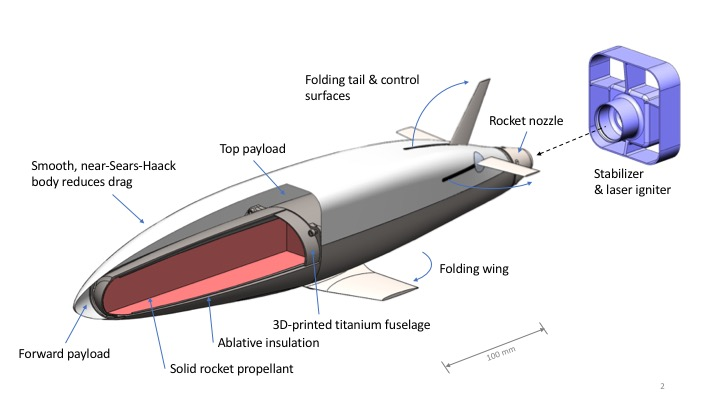
\includegraphics[width=1\textwidth]{vehicle}
    \caption{\label{fig:vehicle} Firefly vehicle cut-away drawing.}
\end{figure}

The motor features segments with different propellant formulations, which is done to control the chamber pressure and thrust. As the burn progresses, the burning surface area changes. Since the chamber pressure and thrust are proportional to the burning surface area, segments of the motor with larger cross-sectional area (near the middle) have a slower burning propellant formulation, and segments with smaller cross-sectional area (near the ends) have a faster burning propellant. The motor has five different propellant segments, each of which needs to be accounted for in the internal ballistics simulator. 

\begin{figure}
    \centering
    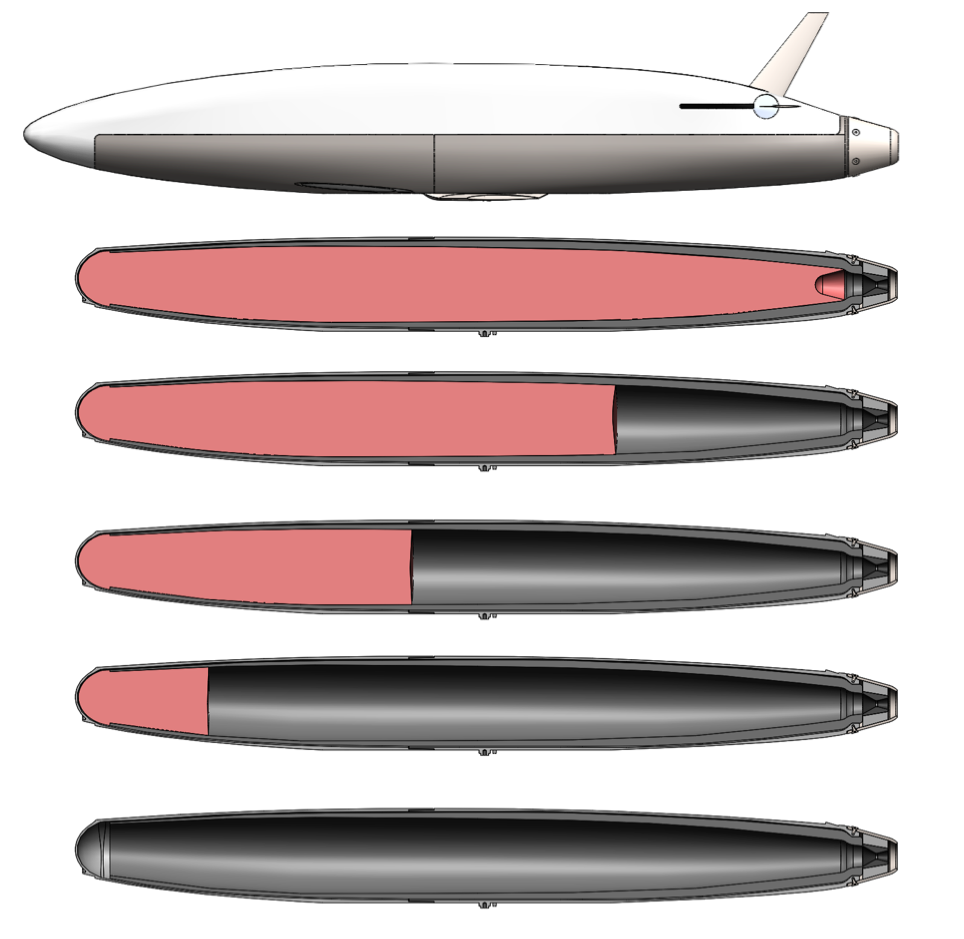
\includegraphics[width=0.6\textwidth]{burn_progress}
    \caption{\label{fig:burn_progress} Progression of motor burn.}
\end{figure}


\section{Equations and Initial Values}

This section will detail the governing system of equations, their derivations, and their initial values. I will first give a summary that lists the modeled variables and equations. Then I will describe their derivations and initial values.

\subsection{Summary of Variables and Equations}

The following values will be modeled with this internal ballistics simulator:

\begin{description}
\item [$p$] chamber pressure
\item [$m$] chamber mass
\item [$V$] chamber volume
\item [$x$] burn distance
\item [$T$] chamber temperature
\item [$c_p$] chamber specific heat
\item [$\frac{1}{\bar{M}}$] chamber molar mass reciprocal
\item [$R$] chamber specific gas constant
\item [$\gamma$] chamber ratio of specific heats
\end{description}

The differential equations implemented in the simulator are as follows:

\begin{align*}
  \frac{dp}{dt} & = \frac{R T}{V} \frac{dm}{dt} - \frac{R T m}{V^2} \frac{dV}{dt} + \frac{m R}{V} \frac{dT}{dt} + \frac{m T}{V}\frac{dR}{dT} \\
  \frac{dm}{dt} &= \frac{dm_{comb}}{dt} - \frac{dm_{exit}}{dt} \\
  \frac{dV}{dt} &= \frac{dx}{dt} A_b(x) \\
  \frac{dx}{dt} &= r = a(x) p^n \\
  \frac{dT}{dt} &= \frac{\left( T_{flame} c_{p, prop} - T c_p \right) \frac{dm_{comb}}{dt}}{m c_p} \\
   \frac{d c_p}{dt} &= \frac{\left( c_{p, prop} - c_p \right) \frac{dm_{comb}}{dt}}{m} \\
    \frac{d \frac{1}{\bar{M}}}{dt} &= \frac{ \left( \frac{1}{\bar{M_{prop}}} - \frac{1}{\bar{M}}\right) \frac{dm_{prop}}{dt}}{m} \\
    \frac{dR}{dt} &= \bar{R} \frac{d \frac{1}{\bar{M}}}{dt} \\
    \frac{d \gamma}{dt} &= \frac{ \left( c_p - R \right) \frac{d c_p}{dt} - c_p \left( \frac{d c_p}{dt} - \frac{dR}{dt} \right)}{\left( c_p - R \right)}
\end{align*}

\subsection{Derivation of Differential Equations}

I am primarily interested in determining the chamber pressure of the motor at all points in time, since this enables the calculation of thrust and flight profile for the Firefly vehicle. To determine the chamber pressure of the motor, we can start with the ideal gas law:

\begin{equation}
  p = \rho R T = \frac{m}{V} R T .
\end{equation}

If we take the derivative of this expressions, we find the following differential equation:

\begin{equation}
  \frac{dp}{dt} = \frac{R T}{V} \frac{dm}{dt} - \frac{R T m}{V^2} \frac{dV}{dt} + \frac{m R}{V} \frac{dT}{dt} + \frac{m T}{V}\frac{dR}{dT} .
\end{equation}

We now determine expressions for each of these derivatives and their dependencies. To determine the mass derivative $\frac{dm}{dt}$, we consider the free volume inside the combustion chamber, and the masses moving in and out of this volume. The mass being added to the free volume by propellant combustion is

\begin{equation}
  \frac{dm_{comb}}{dt} = \rho_{prop} \frac{dV}{dt}.
\end{equation}

The mass flow exiting the volume is dependent on whether the gas flow through the motor's nozzle is choked. If the flow is not choked, then the mass flow is dependent on both the internal chamber pressure and the exit Mach number :

\begin{equation}
  \frac{dm_{exit, unchoked}}{dt} = A_{exit} p \sqrt{\frac{\gamma}{R T}} M \left( 1 + \frac{\gamma - 1}{2} M^2 \right)^{- \frac{\gamma + 1}{2 (\gamma - 1)}}, 
\end{equation}

where the Mach number is determined by

\begin{equation}
  M = \sqrt{ \frac{2}{\gamma - 1} \left( { \left( \frac{p_{exit}}{p} \right)}^{\frac{1 - \gamma}{\gamma}} - 1 \right)}
\end{equation}

If the flow is choked, then the Mach number at the nozzle through is $M = 1$ and the mass flow exiting the chamber is dependent only on the chamber pressure and a few other thermodynamic properties:

\begin{equation}
  \frac{dm_{exit, choked}}{dt} = A_t p \sqrt{\frac{\gamma}{R T}}\left( {\frac{\gamma + 1}{2}} \right)^{- \frac{\gamma + 1}{2 (\gamma - 1)}}
\end{equation}

The rate of change of mass in the combustion chamber is equal to the different between the mass flow entering and exiting the volume of the chamber: 

\begin{equation}
  \frac{dm}{dt} = \frac{dm_{comb}}{dt} - \frac{dm_{exit}}{dt}
\end{equation}

The volume derivative is simply:

\begin{equation}
  \frac{dV}{dt} = \frac{dx}{dt} A_b(x) .
\end{equation}

The burn area $A_b(x)$ can be looked up in a table of values derived from the CAD model of the motor. 

$x$ represents the position of the burning face of propellant as it progresses during the motor burn. The derivative of this position is determined using:

\begin{equation}
  \frac{dx}{dt} = r = a(x) p^n
\end{equation}

This expression comes from Vielle's burn rate law, which says the burn rate $r$ of a propellant is a function of the chamber pressure and two empirically determined values $a$ and $n$. I have determined these values for the propellants in separate experiments for my research. The value $a = a(x)$ is a function of $x$ since $a$ changes with propellant formulation, and the propellant formulation changes as a function of $x$. 

Next I considered the temperature derivative. I assume the combustion chamber is adiabatic, diffusion of the combustion products in the combustion chamber happens very quickly, and that enthalpy is unchanged during the diffusion process. In this case, the rate of temperature change should be proportional to the difference between the flame temperature and the combustion chamber temperature, proportional to the mass flow being added to the chamber due to combustion, and inversely proportional to the mass of gas in the combustion chamber. Combining these thoughts, we can express the temperature derivative as:

\begin{equation}
  \frac{dT}{dt} = \frac{\left( T_{flame} c_{p, prop} - T c_p \right) \frac{dm_{comb}}{dt}}{m c_p}
\end{equation} 

A similar set of assumptions and thoughts can be used to determine the specific heat and molar mass. The rate of change of the specific heat of the gas in the chamber can be expressed as:

\begin{equation}
  \frac{d c_p}{dt} = \frac{\left( c_{p, prop} - c_p \right) \frac{dm_{comb}}{dt}}{m}
\end{equation}

Rather than keep track of the molar mass directly, I keep track of the inverse of the molar mass. Because I am keeping track of the mass of gas in the combustion chamber (rather than the moles of gas), any specific quantity I model must be per kilogram. The rate of change of the reciprocal of molar mass can be expressed as follows:

\begin{equation}
  \frac{d \frac{1}{\bar{M}}}{dt} = \frac{ \left( \frac{1}{\bar{M_{prop}}} - \frac{1}{\bar{M}}\right) \frac{dm_{prop}}{dt}}{m}
\end{equation}

Lastly, we need determine differential equations for the specific gas constant $R$ and the ratio of specific heats $\gamma$. The specific gas constant can be expressed as a function of molar mass:

\begin{equation}
  R = \frac{\bar{R}}{\bar{M}}
\end{equation}

where $\bar{R}$ is the universal gas constant. If we differentiate this, we get

\begin{equation}
  \frac{dR}{dt} = \bar{R} \frac{d \frac{1}{\bar{M}}}{dt}
\end{equation}

The ratio of specific heats $\gamma$ can be expressed as a function of $c_p$ and $R$:

\begin{equation}
  \gamma = \frac{c_p}{c_p - R}
\end{equation}

If we differentiate this expression we find

\begin{equation}
  \frac{d \gamma}{dt} = \frac{ \left( c_p - R \right) \frac{d c_p}{dt} - c_p \left( \frac{d c_p}{dt} - \frac{dR}{dt} \right)}{\left( c_p - R \right)}
\end{equation}

\subsection{Initial Values}

Initial values for the solver are determined based on atmospheric and geometric coniditions of the vehicle before the motor is ignited. The temperature, mass, pressure, density, molar mass reciprocal, specific gas constant, and ratio of specific heats of the gas in the chamber can be determined from atmospheric conditions at 30,000 feet (the altitude at which the vehicle is deployed). We also take the initial burn distance to be 0, and the initial volume is taken as the initial free volume inside the motor. This gives the following list of initial conditions:

\begin{align*}
  p_0 &= 3.009 * 10^4 Pa \\
  m_0 &= 1.38 * 10^{-6} kg \\
  V_0 &= 3 * 10^{-6} m^3 \\
  x_0 &= 0 m \\
  T_0 &= 229 K \\
  c_{p,0} &= 1004 J/kg-K \\
  \frac{1}{\bar{M_0}} &= 34.48 mol/kg \\
  R_0 &= 286.7 J/kg-K \\
  \gamma_0 &= 1.25
\end{align*}

\section{Solvers}

Three explicit numerical schemes were used to evaluate the system of equations: Forward Euler, Runge-Kutta, and Adams-Bashforth. 

\subsection{Forward Euler} 

A simple Forward Euler scheme was implemented as follows:

\begin{equation}
  U_{n + 1} = U_n + \Delta t f_n
\end{equation}

\subsection{Runge-Kutta}

A fourth-order Runge-Kutta scheme was implemented as follows: 

\begin{equation}
  U_{n+1} = \frac{1}{3} \Delta t \left( k_1 + 2 k_2 + 2 k_3 + k_4 \right) + U_n
\end{equation}

where 

\begin{align*}
  k_1 &= \frac{1}{2} f(U_n, t_n) \\
  k_2 &= \frac{1}{2} f(U_n + \Delta t k_1, t_{n + 1/2}) \\
  k_3 &= \frac{1}{2} f(U_n + \Delta t k_2, t_{n + 1/2}) \\
  k_4 &= \frac{1}{2} f(U_n + 2 \Delta t k_3, t_{n + 1})
\end{align*}

\subsection{Adams-Bashforth}

A fourth order Adams-Bashforth scheme was implemented as follows: 

\begin{equation}
U_{n + 1} = \Delta t \left(b_1 f_n + b_2 f_{n-1} + b_3 f_{n-2} + b_4 f{n-3} \right) + U_n
\end{equation}

where

\begin{align*}
  b1 &= 55/24 \\
  b2 &= -59/24 \\
  b3 &= 37/24 \\
  b4 &= -9/24
\end{align*}

The first three time-steps were found using the previously described Runge-Kutta method, since this method looks three time-steps backwards. Then the Adams-Bashforth scheme was implemented for the remaining time steps. 

\section{Results}

Plots of chamber pressure and burn distance versus time are given in Figure \ref{fig:chamber_pressure_compare}. We see decent agreement between the different solvers. 

\begin{figure}
    \centering
    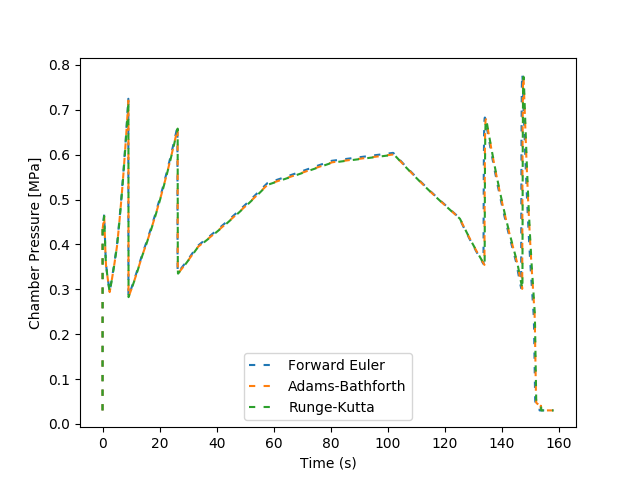
\includegraphics[width=0.85\textwidth]{chamber_pressure_compare}
    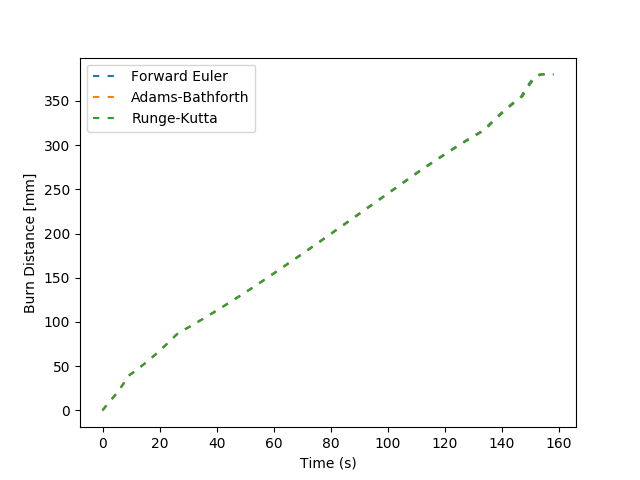
\includegraphics[width=0.85\textwidth]{burn_dist_compare}
    \caption{\label{fig:chamber_pressure_compare} Plots of chamber pressure and burn distance for different solvers.}
\end{figure}


\section{Analysis}
 
\end{document}